\documentclass[../main.tex]{subfiles}

\begin{document}

\textbf{Hatcher 1.3.1.} \par
$\forall x\in A\subset X, \exists U\ni x$ is a neighborhood of $x$ such that $U$ is evenly covered by $p^{-1}(U)\bigsqcup U_{\alpha}$, $\phi_{\alpha}:=p|_{U_{\alpha}}:U_{\alpha}\rightarrow U$ is a homeomorphism with $\psi_{\alpha}$ as its inverse. Then $U\cap A\ni x$ is a neighborhood of $x$ in $A$ such that $\displaystyle{p^{-1}(U\cap A)=p^{-1}(U)\cap p^{-1}(A)=\left(\underset{\alpha}{\bigsqcup}U_{\alpha}\right)\cap \widetilde{A}}=\underset{\alpha}{\bigsqcup}\left(U_{\alpha}\cap \widetilde{A}\right)$, and $\phi_{\alpha}|_{U_{\alpha}\cap \widetilde{A}}=p|_{U_{\alpha}\cap \widetilde{A}}: U_{\alpha}\cap \widetilde{A}\rightarrow U\cap A$ is a homeomorphism with $\psi_{\alpha}|_{U\cap A}$ as its inverse. Hence, $p: \widetilde{A}\rightarrow A$ is a covering space \par
\textbf{1.} \par
\textbf{a)} \par
\textbf{Lemma:} A finite CW complex is Hausdorff and compact. \par
We prove by induction, assume $X$ is a finite CW complex and it is Hausdorff and compact, using $\phi: S^{n-1}\rightarrow X$ to attach $D^{n}$ to $X$, the resulting adjunction space $X\cup_{\phi}D^{n}=X\bigsqcup D^{n} /\sim$, since $X\bigsqcup D^{n}$ is compact, so is $X\cup_{\phi}D^{n}$, for $x\neq y\in X\cup_{\phi}D^{n}$, $\iota_{X}$ is injective by homework 1, thus $\iota_{X}^{-1}(x)\neq\iota_{X}^{-1}(y)$ thus have disjoint neighborhoods in $X$, also, $\iota_{D^{n}}^{-1}(x),\iota_{D^{n}}^{-1}(y)$ are disjoint compact set in $D^{n}$,but $D^{n}$ is a metric space, thus they have disjoint neighborhoods in $D^{n}$, hence $x,y$ has disjoint neighborhood in $X\cup_{\phi}D^{n}$, therefore $X\cup_{\phi}D^{n}$ is Hausdorff
\begin{center}
\begin{tikzcd}
S^{n} \arrow[r,hook,"i"] \arrow[d,"\phi"]
& D^{n} \arrow[d,"\iota_{D^{n}}"] \\
X \arrow[r,hook,"\iota_{X}"]
& X\cup_{\phi}D^{n}
\end{tikzcd}
\end{center}
\textbf{Proposition:} Let $X=X^{n}$ be a finite CW complex, $x_{0}$ is a \(0\)-cell, then the map $\pi_{1}(X^{n-1},x_{0})\rightarrow\pi_{1}(X^{n},x_{0})$ induced by inclusion is surjective where $n\geq 2$ \par
There are finitely many $n$-cells, say $D^{n}_{1},\cdots,D^{n}_{m}$, denote their origin as $O_{1},\cdots,O_{m}$, let $U_{1}:=D^{n}_{1}\setminus\partial D^{n}_{1},\cdots,U_{m}:=D^{n}_{m}\setminus\partial D^{n}_{m},U_{m+1}:=X\setminus \{O_{1},\cdots,O_{m}\}$ is an open cover of $X$, $X^{n-1}$ would be a deformation retraction of $U_{m+1}$, since $X^{n-1},D^{n}_{1}\setminus\{O_{1}\},\cdots,D^{n}_{m}\setminus\{O_{m}\}$ is a close cover of $U_{m+1}$, $X^{n-1}$ is closed because it is compact and $X^{n}$ is Hausdorff, using pasting lemma, define the homotopy $F: U_{m+1}\times I\rightarrow U_{m+1}$ by
\[
\begin{aligned}
F(x,t)&=x, \,\forall x\in X^{n-1} \\
F(x,t)&=(1-t)x+t\dfrac{x}{|x|}, \,\forall x\in D^{n}_{i}\setminus\{O_{i}\}
\end{aligned}
\]
Hence for any loop $\gamma\in\pi_{1}(X^{n},x_{0})$, using Lebesgue's number lemma, we can divide the time into intervals $[s_{j},s_{j+1}]$ so that each interval live inside one of $U_{i}$'s, then the ones that are not contained in $U_{m+1}$ must be contained in some $U_{i}, i\leq m$ and went through $O_{i}$, thus by wiggle it a little we can make $\gamma$ contained in $U_{m+1}$, then compose with the deformation retract, we know that $\gamma$ is homotopic to an element in $\pi_{1}(X^{n-1},x_{0})$ \par
This would imply $\pi_{1}(X^{1},x_{0})\rightarrow\cdots\rightarrow\pi_{1}(X^{n},x_{0})$ is surjective \par
\textbf{Remark:} As it came to me afterwards, I could just define $F: X^{n-1}\bigsqcup_{i=1}^{m}D_{i}^{n}\times I\rightarrow X^{n-1}\bigsqcup_{i=1}^{m}D_{i}^{n}$ by 
\[
\begin{aligned}
F(x,t)&=x, \,\forall x\in X^{n-1} \\
F(x,t)&=(1-t)x+t\dfrac{x}{|x|}, \,\forall x\in D^{n}_{i}\setminus\{O_{i}\}
\end{aligned}
\]
Then $F$ could be factor through the quotient space $X\times I$, thus induce $G: X\times I\rightarrow X^{n-1}\bigsqcup_{i=1}^{m}D_{i}^{n}\rightarrow X\times I$ is a homotopy for the deformation retract \par
\textbf{b)} \par
$S^{1}\vee S^{n}$ could be given a CW complex structure as below with one $0$-cell, one $1$-cell and one $n$-cell
\begin{center}
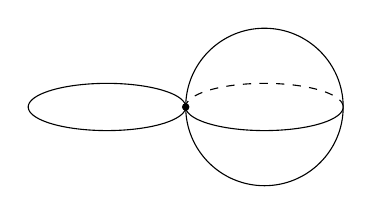
\begin{tikzpicture}
\draw [fill] (0,0) circle [radius=0.04];
\draw (1,0) circle [radius=1];
\draw[dashed] plot[domain=0:pi,smooth,samples=100] ({1+cos(\x r)},{0.3*sin(\x r)});
\draw plot[domain=0:pi,smooth,samples=100] ({1+cos(\x r)},{-0.3*sin(\x r)});
\draw plot[domain=0:2*pi,smooth,samples=100] ({-1+cos(\x r)},{0.3*sin(\x r)});
\end{tikzpicture}
\end{center}
Thus by a), $\mathbb{Z}\cong \pi_{1}(S^{1})\overset{\varphi}{\rightarrow}\pi_{1}(S^{1}\vee S^{n})$ is surjective, then $\pi_{1}(S^{1}\vee S^{n})\cong\pi_{1}(S^{1}) /\ker\varphi$, then $p: X\rightarrow S^{1}\vee S^{n}$ is a covering map, let $H\subset X$ be the helix which is $p^{-1}(S^{1})$, thus by Hatcher 1.3.1. we know $p|_{H}: H\rightarrow S^{1}$ is a covering map, suppose $\ker\varphi\neq 0$, then $\exists \gamma$ such that $0\neq[\gamma]\in\pi_{1}(S^{1},x_{0})$ but $0=[\gamma]\in\pi_{1}(S^{1}\vee S^{n},x_{0})$, suppose $\widetilde{\gamma}$ is a path from $A$ to $B$,such that $p(\widetilde{\gamma})=\gamma$, then $\widetilde{\gamma}$ is a lift of $\gamma$ under either $p|_{H}$ or $p$, by the uniqueness of homotopy lifting, we know that $A\neq B$, but for the same reason, $[\gamma]\neq 0$ in $\pi_{1}(S^{1}\vee S^{n})$ which is a contradiction, thus $\ker\varphi=0$ and  hence $\pi_{1}(S^{1}\vee S^{n})\cong\mathbb{Z}$

\begin{center}
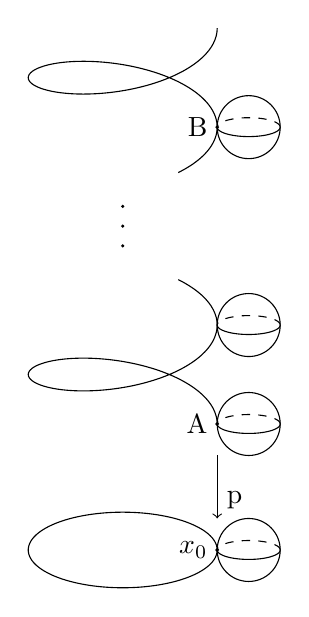
\begin{tikzpicture}[scale=0.4]
\draw plot[domain=-0.3*pi:2*pi,smooth,samples=100] ({-3+3*cos(\x r)},{4+3*pi+0.5*\x+1.2*sin(\x r)});
\draw [fill] (-3,4+2.2*pi) circle [radius=0.03];
\draw [fill] (-3,4+2*pi) circle [radius=0.03];
\draw [fill] (-3,4+1.8*pi) circle [radius=0.03];
\draw [fill] (0,4) circle [radius=0.04];
\draw [fill] (0,4+3*pi) circle [radius=0.04];
\draw [fill] (0,0) circle [radius=0.04];
\node at (0,4)[left] (a){A};
\node at (0,4+3*pi)[left] (b){B};
\node at (0,0)[left] (c){$x_{0}$};
\draw plot[domain=0:2.3*pi,smooth,samples=100] ({-3+3*cos(\x r)},{4+0.5*\x+1.2*sin(\x r)});
\draw (1,4) circle [radius=1];
\draw[dashed] plot[domain=0:pi,smooth,samples=100] ({1+cos(\x r)},{4+0.3*sin(\x r)});
\draw plot[domain=0:pi,smooth,samples=100] ({1+cos(\x r)},{4-0.3*sin(\x r)});
\draw (1,4+pi) circle [radius=1];
\draw[dashed] plot[domain=0:pi,smooth,samples=100] ({1+cos(\x r)},{4+pi+0.3*sin(\x r)});
\draw plot[domain=0:pi,smooth,samples=100] ({1+cos(\x r)},{4+pi-0.3*sin(\x r)});
\draw (1,4+3*pi) circle [radius=1];
\draw[dashed] plot[domain=0:pi,smooth,samples=100] ({1+cos(\x r)},{4+3*pi+0.3*sin(\x r)});
\draw plot[domain=0:pi,smooth,samples=100] ({1+cos(\x r)},{4+3*pi-0.3*sin(\x r)});
\draw[->] (0,3) -- (0,1) node [above right] {p};
\draw (1,0) circle [radius=1];
\draw[dashed] plot[domain=0:pi,smooth,samples=100] ({1+cos(\x r)},{0.3*sin(\x r)});
\draw plot[domain=0:pi,smooth,samples=100] ({1+cos(\x r)},{-0.3*sin(\x r)});
\draw plot[domain=0:2*pi,smooth,samples=100] ({-3+3*cos(\x r)},{1.2*sin(\x r)});
\end{tikzpicture}
\end{center}

\textbf{2.} \par
Let $p: \mathbb{R}\rightarrow S^{1}, t\mapsto \mathrm{e}^{2\pi it}$ be a covering map, and $e_{1}: I\rightarrow S^{1}, t\mapsto \mathrm{e}^{2\pi it}$ be the generator of $\pi_{1}(S^{1},1)$, by homotopy lift we can find $F$ is a lift of $f(e_{1})$, and $1\neq n:=\deg(f)=F(1)-F(0)\in\mathbb{Z}$. Define $G(t):=F(t)-t$, then $G(0)=F(0), G(1)=F(1)-1$, thus $|G(0)- G(1)|=|F(1)-F(0)-1|\geq \left||F(1)-F(0)|-1\right|\geq 1$, since $G$ is continuous, $\exists t\in I$ such that $F(t)-t=G(t)\in\mathbb{Z}$, thus $f\left(e_{1}(t)\right)=p\circ F(t)=p(t)=\mathrm{e}^{2\pi it}=e_{1}(t)$, thus $f$ has a fixed point \par
\textbf{3.} \par
It is easy to show that $g: Y\rightarrow Y, y\mapsto yg$ is a homeomorphism, denote the quotient map as $q$, then for any $q(y)\in Y/G$, since $G$ is a properly discontinuous action on $Y$, there exists a open neighborhood $U$ of $y$ such that $U\cap Ug=\varnothing$, thus $q^{-1}(q(U))=\displaystyle{\bigsqcup_{g\in G}}Ug$ which is open, so is $q(U)$, and also $q|_{Ug}$ is continuous, injective and surjective, for any open set in $Ug$ which would have the form $Ug\cap Vg=(U\cap V)g$ where $V$ is open in $Y$, $q|_{Ug}((U\cap V)g)=U\cap V$ is open, thus $q|_{Ug}$ is also open, hence a homeomorphism. Therefore $q$ is indeed a covering map

\end{document}